\section{Methodology and Our Approach}
\label{sec:povm}


\para{Quantum State Discrimination (QSD).} 
Given a quantum state $\ket{\phi}$ that is known to be equal to one of the 
states (known as \emph{target states}) in the set 
$\{\ket{\phi_1}, \ket{\phi_2}, \ldots, \ket{\phi_n} \}$,
the quantum state discrimination (QSD) problem 
is to determine which state $\ket{\phi}$ really is.
In general, each target state $\ket{\phi_i}$ may be associated with
a prior probability $q_i$; in this paper, we assume uniform
prior.
%%%%%%%%%%%%%%%%%%
The QSD problem is typically solved using a series of measurements or 
a single measurement---as defined below.
%%%%%%%%%%%%
It is known that if the target states $\{\ket{\phi_i}\}$  are not mutually orthogonal, 
then there is no quantum measurement capable of perfectly (without error)
distinguishing the states.
Thus, a QSD solution may give an erroneous answer---i.e., guess the
state to be in $\ket{\phi_i}$ when the state is really in $\ket{\phi_j}$ for 
some $i \neq j$. Thus, a QSD solution is associated with an overall {\em probability
of error} (PoE), and the optimization goal of the QSD problem is to determine the
measurement (or a sequence of measurements) that minimizes the PoE. 
We note that in our developed schemes, we don't actually solve the QSD 
problems that
arise due to the impracticality of implementing the general POVMs, as discussed
later; instead,
we just use the standard POVM known as pretty good measurement (PGM).

\softpara{General Measurements.} 
A general measurement~\cite{qcqi-book} is defined by matrices $M_1, M_2, \ldots, M_n$ such that
$\sum_i M_i^{\dagger}M_i = I$ where $M_i^{\dagger}$ is the conjugate transpose of
$M_i$. If this general measurement is carried out on a pure state,
%\footnote{See~\cite{qcqi-book} for generalization to mixed states} state $\ket{\phi}$
we see the outcome ``$i$'' with 
probability $p(i) = \bra{\phi}M_i^{\dagger}M_i\ket{\phi}$. Thus, if we associate
the outcome ``$i$'' with the given state $\ket{\phi}$ being in the target state 
$\ket{\phi_i}$, the probability of error (PoE) for the given measurement $\{M_i\}$
is given by $\sum_i \sum_{j \neq i} \bra{\phi_i}M_j^{\dagger}M_j\ket{\phi_i}$.

If we are only interested in the probability of outcomes (as in our context), the above
general measurement can also be represented by the set of positive semi-definite 
matrices (PSD) $\{E_i = M_i^{\dagger}M_i\}$ where $\sum_{i} E_i = I$. This representation 
is called positive-operator valued measure (POVM); in this paper, we use this 
representation of measurement for simplicity. 

% The above measurement can also be repre
% Mathematically, a POVM is a set of positive semi-definite Hermitian matrices 
% $\{E_i\}$ on a Hilbert space $\mathcal{H}$ that sum to the 
% identity matrix, i.e., 
% $\sum_{i} E_i = I$.
% In quantum mechanics, the POVM element $\{E_i\}$ is associated with the measurement outcome $i$, such that the probability of obtaining it when making a measurement on the quantum state $\rho$ is
% \begin{equation}
%     Prob(i) = tr(\rho E_i) = tr(\ket{\psi} \bra{\psi} E_i)
% \end{equation}
% where $tr$ is the trace operator, and $\rho = \ket{\psi} \bra{\psi}$ for pure states.
% \blue{What is probability of error? Focus on pure states?}


\para{Core Idea: TX Localization as QSD.}
Consider a geographic area where a transmitter can be at a set of potential locations $\{l_1, l_2, \ldots, l_n\}$. 
For simplicity, let us assume that the transmission power is constant.
%%%%%
Let the initial state of the quantum system, composed of say $m$ distributed quantum sensors,
be $\ket{\psi_0}$. 
When the transmitter $T$ is at a location $l_i$, let the impact of the $T$'s transmission from location $l_i$ evolve the overall state of the quantum system to $\ket{\psi_i}$ 
based on the model described in the previous section.
%%%%%%%%%%%%%%%
Now, consider the set of target states $\{\ket{\psi_1}, \ket{\psi_2}, \ldots, \ket{\psi_n}\}$ corresponding to the set of potential locations of the transmitter. Then, localizing the transmitters, i.e., determining the location $l_i$ from where the transmission occurred, is
tantamount to solving the QSD problem with the target states $\{\ket{\psi_i}\}$.
Thus, determining the state of the quantum system yields
the transmitter location.

\softpara{Selection of Initial State and Measurement.} 
In the above context, our goal is to select an initial state $\ket{\psi_0}$ and the 
POVM measurement (i.e., PSD matrices $\{E_1, \ldots, E_n\}$, one for each potential outcome/location) such that the overall \eat{probability of error} PoE is minimized --- for a given setting of transmitter location, quantum sensors, and signal propagation model.
%%%%%%%%%%%%%%%%%%%%%%%%%%%%%%%%%%%%%
%%%%%%%%%%%%%%%%%%%%%%%%%%%%%%%%%%%%%
The optimization problem of selecting an optimal combination of initial state and POVM
in our context is beyond the scope of this work. Here, we use a non-entangled uniform superposition
pure initial state $\ket{\psi_0} = \sum_{i=0}^{2^m-1} \frac{1}{\sqrt{2^m}} \ket{i} $. 
%%%%%%
For a given initial state and target states, determining an optimal POVM can be shown to
be a convex optimization problem and can be solved using an appropriate semi-definite program (SDP)~\cite{semidefinite}. However, due to scalability challenges in solving the
SDP, whose size is exponential in the number of quantum sensors involved, 
in this paper, we use
a well-known measurement known as {\em pretty-good-measurement} (PGM) which is known to
perform well in general settings~\cite{prettygood}. The PGM POVM is given by: 
\begin{equation}
    E_i = q_i {\rho}^{-1/2} \rho_i {\rho}^{-1/2}
    \label{eqn:pgm}
\end{equation}
where $q_i$ is the prior probability and $\rho_i = \ket{\psi_i}\bra{\psi_i}$ is the {\em density matrix} of the $i^{th}$ target state $\psi_i$, and  $\rho = \sum_{i} q_i \rho_i$. 

\begin{figure}
    \centering
    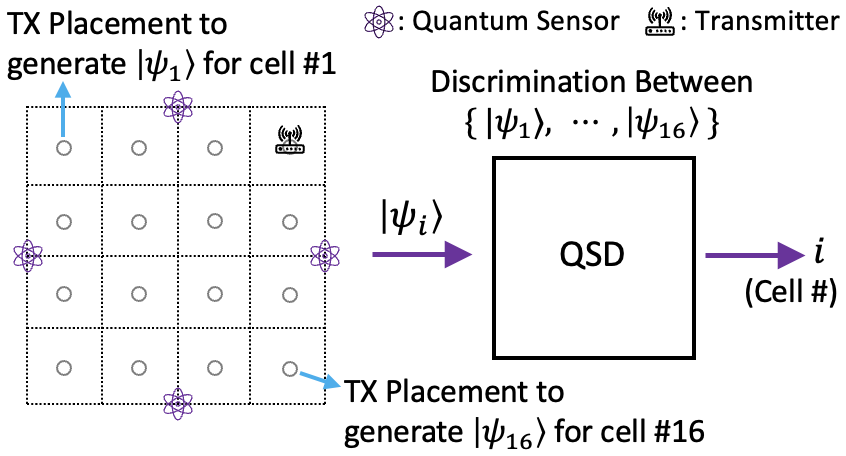
\includegraphics[width=0.8\textwidth]{chapters/qce/figures/onelevel.png}
    \caption{\povmone Scheme.}
    \label{fig:onelevel}
\end{figure}



\para{Basic \povmone Scheme; Key Challenges.}
The above-described methodology is essentially our basic \povmone localization scheme, see Fig.~\ref{fig:onelevel}. 
That is, the \povmone scheme localizes the transmitter by first determining the set 
of target states $\{\ket{\psi_1}, \ket{\psi_2}, $ $ \ldots, \ket{\psi_n}\}$ corresponding 
to the centers of the cells (a set of transmitter locations), and then, localizes the 
transmitter
in real-time by performing QSD over the evolved quantum state using PGM measurement.
Note that we use only the cells' centers to generate the target states, and also that
the predicted location
of the transmitter is always a cell's center in the QSD-based schemes, since the QSD-based
schemes are fundamentally classification of the transmitter location into cells.
{\em However, during evaluation, the actual
location of the transmitter can be anywhere in the area}---presumably, non-center locations 
of the transmitter may incur higher localization errors.

%%%%%%%%
% \CZ{Is this assumption still necessary?}We assume that the only potential locations of the transmitter are the centers of 
% the cells of the grid (we relax this assumption in Section~\ref{sec:eval}).
%%%%%%%%%%%%%%%
The key challenges in the \povmone scheme are twofold: (i) It is likely to incur a high probability
of error due to a large number of target states (equal to the number of potential 
transmitter locations). (ii) A global POVM measurement over a large number of sensors can be
difficult to implement in practice~\cite{pra19-povm}; even ignoring the communication cost of teleporting the 
qubits to a central location, the main challenge arises due to the complexity of the circuit or
hardware required  to implement a POVM over a large number of qubit states.
%%%%%
We address these challenges by designing a two-level localization scheme as described below; 
in the following section, we further address the above challenges by designing non-QSD based
schemes.

% But we observe that a POVM having too many outputs will lead to lower accuracy.
% Because when the number of quantum states is high, the difference between each state is relatively smaller (i.e., the overlap between quantum states  is relatively larger). 
% Thus being more difficult to discriminate.
% So we want to avoid  a POVM that has hundreds of elements.
% 2) The second challenge is that if we do a global measurement on a relatively high number of sensors, the dimension of the Hilbert space will be large.
% It results in POVM elements being too costly in RAM during computation.
% Take an example of doing a global measurement on 12 sensors.
% Each POVM element will be a complex number matrix of dimension $2^{12} \times 2^{12}$.
% Each complex number needs 16 bytes.
% A POVM of 256 elements will cost 69 GB of RAM.
% In reality, the physical implementation of POVM is costly as well~\cite{pra19-povm}.
% So we want to avoid doing a global POVM on tens of sensors.
% But if we actually do have tens of quantum sensors, not being able to use all of them is a waste of resources.


\para{\povm Scheme}. 
% A quantum counterpart of the fingerprinting-based approach has a training phase and a localization phase.
% \povm is our approach for the localization phase.
% The names come from the critical role POVM plays in the approach.
% The two challenges mentioned in the previous paragraph can be summarized as the scalability challenge.
\povm solves the above-mentioned challenges by localizing the transmitter by using two levels
of POVMs, with each POVM requiring a measurement over a much fewer number of sensors and with a much fewer number of 
possible target states. 
%%%%%%%%%
We discretize the given area into a grid; each unit of the grid is called a \emph{cell}. 
A \emph{block} is a group of neighboring cells that form a rectangle. 
In Fig.~\ref{fig:twolevel} (a), a grid has $4\times 4$ cells and $2\times 2$ blocks. 
The thick dotted lines depict the blocks while the non-thick dotted lines depict the cells.
In general, for a $N \times N$ grid with $N^2$ cells, we construct blocks by dividing the entire grid
into $\sqrt{N} \times \sqrt{N}$ blocks --- yielding $N$ blocks in the whole area, with each block comprised of $ \sqrt{N} \times \sqrt{N} = N$ cells. Without loss of generality, we assume $\sqrt{N}$ to be an integer in our discussion.
%%%%%%%%%%%%%%%%%%%%%%
The basic idea of the \povm scheme
is to localize the transmitter in two stages: first, localize the transmitter at a block level (Fig.~\ref{fig:twolevel} (a)); and then, within that block, localize the transmitter at the cell level (Fig.~\ref{fig:twolevel} (b)). The sensors, target states, and POVMs used for localization at these two stages are different. Such a two-stage localization scheme naturally addresses the above-mentioned challenges by reducing both the number of sensors as well as target states required at 
each stage. We describe the scheme in more detail below.
%%%%%%%%%%%%%%%%%%%



\begin{figure*}[t]
    \centering
    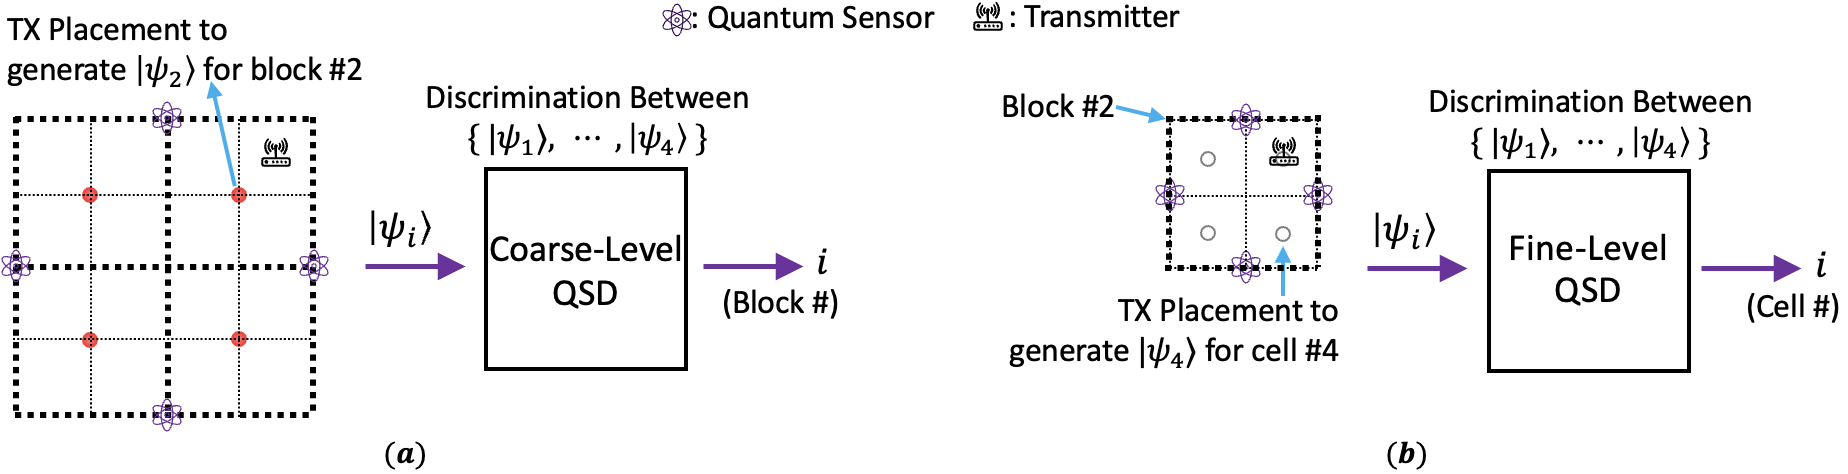
\includegraphics[width=0.99\textwidth]{chapters/qce/figures/twolevel.png}
    \caption{\povm Scheme. (a) Coarse-level localization phase, and (b) Fine-level localization phase.}
    \label{fig:twolevel}
\end{figure*}

\softpara{Coarse-Level Localization.} 
The coarse level concerns localizing the transmitter at the block level, and is done based on {\em coarse-level sensors} deployed over the entire given area. The target states for the coarse-level QSD/localization are the states corresponding to the location at the center of each block in the given area. As mentioned above, since the number of blocks is $N$, the number of target states for the Coarse-Level localization is $N$. The POVM measurement for the coarse-level localization is constructed using 
Eqn.~\ref{eqn:pgm} for the PGM measurement over the target states derived from the impact of 
the transmitter at coarse-level discrete locations (i.e., the center of the blocks) on the coarse-level sensors.
Note that in reality, the transmitter is likely not at the center of the blocks---but, we stipulate that a block's center is a reasonable representative of the actual locations of the transmitter in that block.
%%%%%%%%%%%%%%
More formally, let $\{L_1, L_2, \ldots, L_N\}$ denote the centers of the blocks in the
area, and $S$ be the coarse-level sensors. Let $\hat{U}_i$ denote the impact on $S$ when the transmitter is at location $L_i$. Then, the target states for the coarse-level localization 
are $\{\hat{U}_i \ket{\psi_0}\}$ where $\ket{\psi_0}$ is the initial state of $S$. 
These target states are used to determine the POVM measurements as per Eqn.~\ref{eqn:pgm}, and thus, determine the block.


\softpara{Fine-Level Localization.}
Once the transmitter has been localized within a block $B$ via coarse-level localization, the 
transmitter is then localized at a cell level within $B$. For fine-level localization, each block $B$ has a set of fine-level sensors $S(B)$ deployed within $B$ (which need not be 
disjoint from the coarse-level sensors). 
The target states for fine-level localization within $B$ correspond 
to the potential locations of the transmitter within $B$ which are the centers
of the cells within $B$, see Fig.~\ref{fig:twolevel} (b), and is derived from the impact of the transmitter's signal at
the fine-level sensors $S(B)$. 
%%%%%%%%%%%%%%%%%%%%%%
Note that at the fine-level localization phase, only the sensors $S(B)$ where $B$ is the block selected in the previous coarse-level localization are involved. Note that $S(B_1)$ and $S(B_2)$ from two different blocks need not be disjoint. 
\eat{since sensors only their common border could be involved in fine-level localization within both blocks.}
%%%%%%%%%%%%
More formally, let $\{l_1, l_2, \ldots, l_N\}$ denote the centers of the cells in the
block $B$ selected by the coarse-level localization phase, and $S(B)$ be the fine-level sensors. Let $\hat{U}_i$ denote the impact on $S(B)$ when the transmitter is at location $l_i$. Then, the target states for the fine level localization 
are $\{\hat{U}_i \ket{\psi_0}\}$ where $\ket{\psi_0}$ is the initial state of $S(B)$. These target states
are used to determine the POVM measurement as per Eqn.~\ref{eqn:pgm}, and thus, determine
the cell within the block $B$, which is the TX location. 
As mentioned before in the one-level scheme, we note that, during evaluation, the location of the transmitter can be anywhere in 
the area, even though we have only use the cells' centers to generate the target states.

\eat{For the sensor deployment, the sensors will be randomly spread out, ideally close to uniform to better cover the whole area.}



\eat{
\softpara{Psuedo Code Description.}
Algorithm~\ref{algo:povm-loc} is the pseudo-code of \povm.
Algorithm~\ref{algo:povm-loc} relies on Procedure~\ref{algo:sense-measure} that repeats the process of the quantum sensor network preparing the state and the quantum measurement.

\begin{algorithm}[h] 
  	\KwIn{$\{cE_i\}$ -- one coarse-level POVM}
        \KwIn{[$\{fE_i^{0}\}, \{fE_i^{1}\}, \cdots$] -- an array of fine-level POVMs}
	\KwOut{location $(x, y)$}
        $repeat \leftarrow$ 1000 \;	
        $j \leftarrow$ SenseMeasure($\{cE_i\}$, $repeat$) \;
        $block_j \leftarrow$ the block associated with $j$ \;
        $\{ fE_i\} \leftarrow$ the fine-level POVM associated with $block_j$ \;
        $j \leftarrow$ SenseMeasure($\{fE_i\}$, $repeat$) \;
        $cell_j \leftarrow$ the cell associated with $j$ \;
        % \uIf{$cell_j$ is at the edge of two blocks}{
        %     $block_e \leftarrow$ the block that covers the edge of the two blocks \;
        %     $\{ fE_i\} \leftarrow$ fine-level POVM associated with $block_e$ \;
        %     $j \leftarrow$ SenseMeasure($\{fE_i\}$, $repeat$) \;
        %     $cell_j \leftarrow$ the cell associated with $j$ \;
        % }
        \Return the location $(x, y)$ of $cell_j$ \;
	\caption{\povm}
\label{algo:povm-loc}
\end{algorithm}
\begin{procedure}[h]
    \KwIn{$\{E_i\}$ -- a POVM}
    \KwIn{$K$ -- number of repetition}
    \KwOut{the most frequent measurement outcome}
    $count \leftarrow$ a key-value pair dictionary\;
    $qsensors \leftarrow$ a set of quantum sensors associated with the POVM $\{E_i\}$ \;
    \For{$k=1 \cdots K$}{
        $\rho \leftarrow $ a quantum state sensed by $qsensors$ \;
        $i \leftarrow$ outcome of measuring $\rho$ via POVM $\{E_i\}$ \;
        $count[i] =  count[i] + 1$ \;
    }
    \Return $ arg\,max_{\{ i\}} \ count[i]$ \;
    \caption{SenseMeasure($\{E_i\}$, $K$)}
\label{algo:sense-measure}
\end{procedure}
}

% \para{\povmpro Scheme.\CZ{consider remove this part}} The above described \povm scheme addresses the scalability challenges sufficiently, and also works reasonably well in practice as observed in our evaluations.  However, we also observed in our evaluations that the \povm scheme has a high error rate when the transmitter is situated at the edge of the blocks; this is unsurprising as a transmitter on either side of a block's borders (i.e., on different blocks, but at the block edge) is likely to have a similar impact on the sensors. See
% Fig.~\ref{fig:twolevel-pro} (a). 
% %%%%%%%%%%%%%%%%%%%%%%%%%%%%
% %Another observation is that the wrong output cell of \povm is usually nearby to the correct cell, like the other side of the border.
% To circumvent such types of errors, we add an additional phase to \povm where we 
% re-localize a transmitter that has been localized in at the edge blocks by \povm. 
% %%%%%%%%
% We refer to this scheme as \povmpro. 
% %%%%%%%%%%
% In essence, \povmpro consists of \povm's coarse and fine-level localization phases and an additional fine-level localization phase (called a {\em border-level} localization phase) where we create new blocks referred to as {\em border-blocks} that cover the border of the original blocks. See Fig.~\ref{fig:twolevel-pro} (b). Each border-block $B'$ is associated with its own set of fine-level sensors $S(B')$, which as before need not be disjoint from sets of fine-level sensors of other blocks or border-blocks.
% %%%%%%%%%%%%%%%%%%%%%%
% Localization within a border-block $B'$ is done similar as before---i.e., target states
% are created corresponding to centers of cells within $B'$ and an appropriate QSD solution
% used to localize the transmitter within $B'$. See Fig.~\ref{fig:twolevel-pro} (b).


\softpara{Multi-shot Discrimination.}
The quantum measurement is intrinsically probabilistic and the single-shot discrimination can incur a high probability of error. One way to reduce this probability of error is to repeat the 
discrimination process many times and pick the most frequent measurement outcome. 
%%%%%%%%%%%%%
Such repeated measurements are commonly done in quantum sensing~\cite{RevModPhys.quantumsensing} and computing~\cite{Shor_1997}.
%%%%%%
In our context, the repetitions are done while the transmitter remains fixed.


%which will require the quantum state to be prepared by the QSN multiple times and measured multiple times in the localization schemes.

%We repeat 1000 times and return the most frequent measurement outcome, which in most cases is the correct location.

\eat{This repetition is applied to the \povmone, the coarse/fine level of \povm, and also the \povmpro in the following paragraphs.}
